\documentclass{beamer}
\usepackage{multicol}
\usepackage{array}
\usepackage{siunitx}
\setbeamertemplate{footline}[frame number]
\usepackage{float}
\usepackage{comment}
\usepackage{gensymb}
\usepackage{setspace}
\usepackage[english]{babel}
\usepackage[utf8x]{inputenc}
\usepackage{amsmath}
\usepackage{amssymb}
\usepackage{tabularx,ragged2e,booktabs,caption}
\usepackage{longtable}
\usepackage{mathtools}
\usepackage{empheq}
\usetheme{Rochester}
\usecolortheme{whale}
\usepackage{tikz}
\usetikzlibrary{shapes.geometric, arrows}
\tikzstyle{squ} = [rectangle, rounded corners, minimum width=1.5cm, minimum height=1.5cm, text centered, draw=black]
\tikzstyle{arrow} = [thick,->,>=stealth]

\title{\small{An Age Structured Model of the Impact of Buffelgrass on Saguaro Cacti and their Nurse Trees}}

\author{Lucero Rodríguez-Rodríguez\inst{1} \and Erin Stafford\inst{2}\\
\and Anna Williams\inst{3}\and and  Brian Wright\inst{4}}
 
\institute
{
  \inst{1}University of Texas Rio Grande Valley
  \and
  \inst{2}Tulane University
  \and
  \inst{3}University of Texas at Austin
  \and
  \inst{4} University of Redlands
}
%\titlegraphic{ \vspace{-4cm} \hspace{8cm} \includegraphics[width=2cm]{MTBILogo.png}}
\date{\today} 
\begin{document}

\begin{frame}
  \titlepage
\begin{center}
\vspace{-2cm} \hspace{8cm} \includegraphics[scale=.1]{MTBILogo.png}
\end{center}
\end{frame}

\section{Introduction}

\begin{frame}{Importance of the Saguaro Cactus}

\begin{minipage}{0.49\textwidth}
\begin{figure}[center]
\includegraphics[scale=3]{saguaro3.JPG}\\
\tiny{www.sonorandesert.org/2011/09/29/semptember-29th-2011-enewsletter/}
\end{figure}
\end{minipage}
\hfill
\begin{minipage}{0.49\textwidth}
\footnotesize{\begin{itemize}
\item The saguaro cactus, or {\it{Carnegiea gigantea}}, is a \textbf{keystone species} of the Saguaro National Park.
\item<2-> The saguaro serves as a \textbf{habitat} and \textbf{food source} for many other species in the region.
\item<3-> Changes in the saguaro cactus population indicate the \textbf{health of the  ecosystem}. 
\item<4-> The saguaro is also important for the \textbf{tourism industry} and has \textbf{cultural significance} to the Papago and Pima nations.
\end{itemize}}
\end{minipage}
\end{frame}

\begin{frame}{Palo Verdes, Nurse Trees of the Saguaro}

\begin{minipage}{0.49\textwidth}
\begin{figure}[center]
\includegraphics[scale=0.2]{saguaro-nurse-tree.jpg}\\
\tiny{www.wildsonora.com/image-content/saguaros-and-nurse-tree}
\end{figure}
\end{minipage}
\hfill
\begin{minipage}{0.49\textwidth}
\small{\begin{itemize}
\item The palo verde serves as a \textbf{nurse tree} for juvenile saguaros.
\item<2-> Nurse trees \textbf{increase} the chance of \textbf{germination} and \textbf{survival} for juvenile saguaros.
\item<3-> When saguaros mature to a point where they no longer need the cover of the nurse tree, they begin to \textbf{compete} with the trees.
\item<4-> A palo verde typically \textbf{cannot out-compete} a saguaro.
\end{itemize}}
\end{minipage}
\end{frame}

\begin{frame}{The Danger of Buffelgrass}
\begin{minipage}{0.49\textwidth}
\begin{figure}[center]
\includegraphics[scale = 0.4]{buffelgrass.jpg}\\
\tiny{www.desertmuseum.org/invaders/invaders\_buffelgrass.php}
\end{figure}
\begin{figure}[center]
\includegraphics[scale = 0.85]{buffelgrassfire.jpg}\\
\tiny{www.nps.gov/articles/buffelgrass-management-saguaro.htm}
\end{figure}
\end{minipage}
\hfill
\begin{minipage}{0.49\textwidth}
\small{\begin{itemize}
\item In 1989, buffelgrass was introduced to Saguaro National Park.
\item<2-> Buffelgrass is an \textbf{invasive species} able to grow in close proximity to other plants.
\item<3-> Buffelgrass,a \textbf{fire-adapted plant}, is able to survive fires and quickly regrow.
\item<4-> Buffelgrass acts as a \textbf{fuel for fires}, quickly burning native plants like saguaros and nurse trees and replacing them within weeks.
\end{itemize}}
\end{minipage}
\end{frame}

\begin{frame}{The Saguaro Population has Begun to Decline}
\begin{center}
\begin{figure}
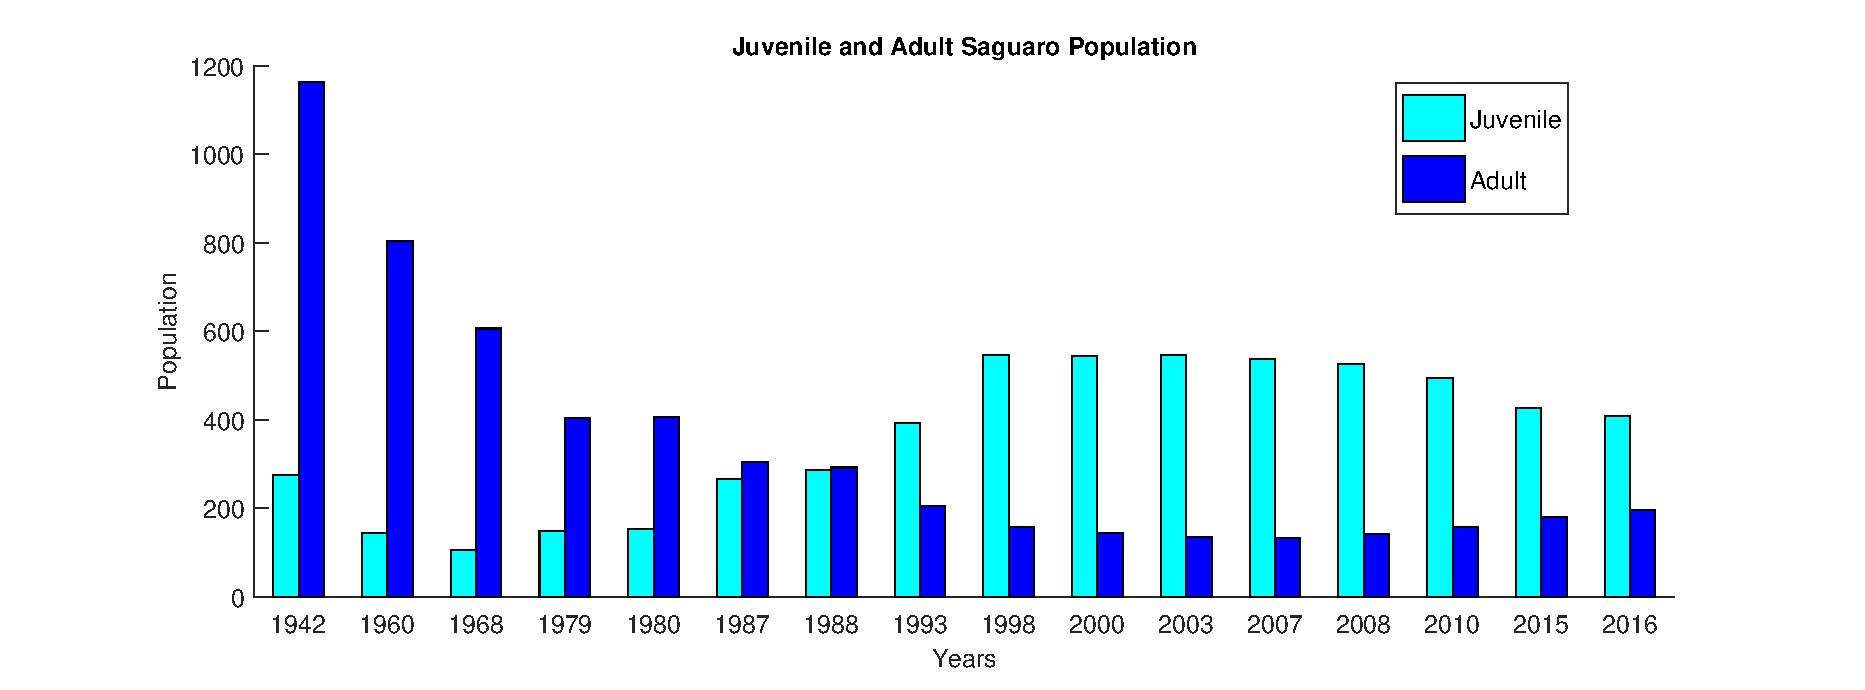
\includegraphics[scale=.37]{sagpop.eps}
\end{figure}
\end{center}
\small{Data provided by Orum et.al. shows the changes in the distribution of adult and juvenile saguaro populations from 1942 to 2016 \cite{OrumData}.}
\end{frame}

\begin{frame}{The Question}
\textbf {Under what conditions will buffelgrass propagated wildfires interrupt the natural life cycle between the saguaro cactus and its nurse trees?}
\newline\newline
\begin{minipage}{0.15\textwidth}
\begin{figure}
\includegraphics[scale=.42]{SaguaroandNurse1.jpg}\\
\tiny{www.pamperingca
mpers.wordpress. com/tag/saguaro}
\end{figure}
\end{minipage}
\hfill
\begin{minipage}{0.05\textwidth}
\includegraphics[scale = 0.1]{plus-sign.jpg}
\end{minipage}
\hfill
\begin{minipage}{0.2\textwidth}
\begin{figure}
\includegraphics[scale = 0.6]{buffelgrassfire.jpg}\\
\tiny{www.desertmuseum.org/invader s/invaders\_buffelgrass.php}
\end{figure}
\end{minipage}
\hfill
\begin{minipage}{0.1\textwidth}
\includegraphics[scale = 0.2]{equal.png}
\end{minipage}
\hfill
\begin{minipage}{0.2\textwidth}
\includegraphics[scale = 0.03]{Question_mark.png}
\hfill
\end{minipage}
\vskip .5cm
%The observations made during the past 75 years suggest that the success of the Saguaros’ s regeneration in the 21st  century will depend on a combination of factors including nurse plant quality, climate, and fire associated with the invasive buffelgrass.
\end{frame}

\begin{frame}{Assumptions of the Model}
%The populations under study in this model include saguaros, palo verdes, and buffelgrass. The interactions of interest between these populations that are considered in the model are as follows:
\begin{itemize}
\item Juvenile saguaros are in the age range of 1 to 35, while the natural life span of all adult saguaros is on average 175 years.
\item<2-> Nurse trees do not out compete adult saguaros for resources. However, juvenile saguaros compete over space with adult saguaros.
\item<3-> Nurse trees increase the available space for juvenile saguaros.
\end{itemize}
\end{frame}

\begin{frame}{Flow Chart Diagram of the Model}
Species interactions:
\begin{itemize}
\item Commensalism between juvenile saguaros and nurse trees
\item Competition between adult saguaros and nurse trees
\item Buffelgrass propagated wildfire.
\end{itemize}
\begin{figure}
    \begin{center}
    \tiny{
        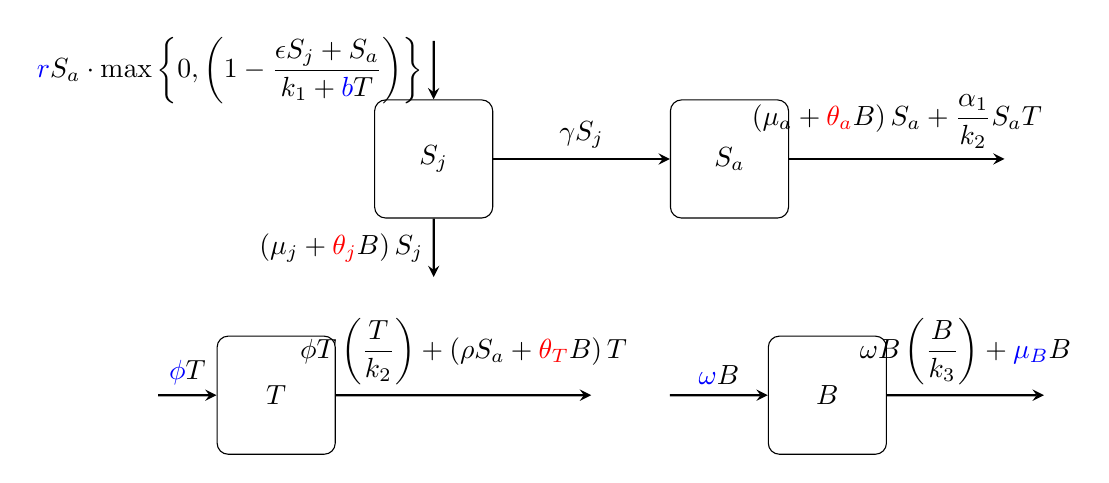
\begin{tikzpicture}[scale = 0.5,node distance=1cm]
        \node (eq1) [squ, xshift = -4cm,yshift=-1cm] {$S_j$};
        \node (eq2) [squ, right, xshift=-1cm, yshift=-1cm] {$S_a$};
        \draw [arrow] (eq1) -- node[anchor=south] {$\gamma S_j$}(eq2);
        \node (eq3) [squ, xshift=-6cm, yshift=-4cm] {$T$};
        \node (eq4) [squ, xshift = 1cm, yshift = -4 cm]{$B$};
        \coordinate (plain1) at (-8,1) {};
        \draw [arrow] (plain1)--node[anchor=east]{$\textcolor{blue}{r} S_a\cdot\text{max}\left\lbrace0,\left(1-\displaystyle\frac{\epsilon S_j + S_a}{k_1 + \textcolor{blue}{b} T}\right)\right\rbrace$}(eq1);
        
        \coordinate (plain2) at (-8,-5){};
        
        \draw[arrow](eq1)--node[anchor=east]{$\left(\mu_j + \textcolor{red}{\theta_j} B\right)S_j$}(plain2);
        
        \coordinate (plain3) at (6.5,-2){};
        \draw [arrow](eq2)--node[anchor=south]{$\left(\mu_a + \textcolor{red}{\theta_a} B\right)S_a + \displaystyle\frac{\alpha_1}{k_2} S_a T$}(plain3);
        
        \coordinate(plain4) at (-4,-8){};
        \draw [arrow](eq3)--node[anchor=south]{$\phi T \left( \displaystyle\frac{T}{k_2}\right) + \left(\rho S_a + \textcolor{red}{\theta_T} B\right) T$}(plain4);
        
        \coordinate(plain5) at (-15,-8){};
        \draw[arrow](plain5)--node[anchor=south]{$\textcolor{blue}{\phi} T$}(eq3);
        
        \coordinate (plain6) at (-2,-8){};
        \draw[arrow](plain6) -- node[anchor = south]{$\textcolor{blue}{\omega} B$}(eq4);
        
        \coordinate(plain7) at (7.5,-8){};
        \draw[arrow](eq4) -- node[anchor = south]{$\displaystyle\omega B\left(\frac{B}{k_3}\right) + \textcolor{blue}{\mu_B} B$}(plain7);
        \end{tikzpicture}
        }
    \end{center}
    \label{fig:tikz}
\end{figure}
\end{frame}

\begin{frame}{Parameters of the Model}
Parameter values were estimated through review of existing literature.
\begin{center}

\setlength{\arrayrulewidth}{.3mm}
%\setlength{\tabcolsep}{20pt}
\renewcommand{\arraystretch}{1.5}


{\tiny \begin{tabular}{ |p{1cm}|m{3cm}| p{1cm}| p{3cm}|}

\hline
Parameter & Description & Parameter & Description\\
\hline
$\textcolor{blue}{r}$ & Germination rate & $k_1$& Adult saguaro carrying capacity\\
\hline

$\epsilon$ & Converts juveniles to adults & $\textcolor{blue}{b}$ & Average juveniles under nurse tree\\
\hline

$\gamma$& Maturation rate & $\mu_j$ & Juvenile death rate\\
\hline

$\alpha_1$& Saguaro death rate by competition & $k_2$ & Carrying capacity of adults and trees\\
\hline

$\mu_a$ & Adult death rate & $\textcolor{blue}{\phi}$ & Growth tree population\\
\hline
$\rho$ & Tree competition death rate & $\sigma$ & Proportion carrying capacity\\
\hline
$\textcolor{red}{\theta_j}$ & Grass fire frequency effect-juvenile& $\textcolor{red}{\theta_a}$ & Grass fire frequency effect-adult\\
\hline
$\textcolor{red}{\theta_t}$ &Grass fire frequency effect-tree & $\textcolor{blue}{\omega}$ & Grass growth rate\\
\hline
$\mu_B$ & grass harvesting & $k_3$ & Carrying capacity of grass\\
\hline
\end{tabular}}
\end{center}
\end{frame}

\begin{frame}{The Model}
%\begin{subequations}
\begin{equation*}
\displaystyle\frac{dS_j}{dt}= rS_a\cdot \text{max}\left\lbrace0,\left(1-\displaystyle\frac{\epsilon S_j + S_a}{k_1+b T}\right) \right\rbrace - \gamma S_j - \mu_j S_j - \theta_j B S_j ,
\end{equation*}

\begin{equation*}
\displaystyle\frac{dS_a}{dt} = \gamma S_j -\displaystyle\frac{\alpha_1}{k_2}S_a T - \mu_a S_a - \theta_a B S_a ,
\end{equation*}

\begin{equation*} \label{eqBuffel}
\displaystyle\frac{dT}{dt} = \phi T\left(1 - \displaystyle\frac{T}{k_2}\right) - \rho S_a T - \theta_T B T ,
\end{equation*}

\begin{equation*}
\displaystyle\frac{dB}{dt} =\omega B \left(1-\displaystyle\frac{B}{k_3}\right) - \mu_B B
\end{equation*}
{\small Buffelgrass grows independently of nurse trees and saguaros, so the model can be redimensionalized into a 3 compartment system by redefining 5 parameters, $\mu_j$, $\mu_a$, $\phi$, $k_2$, and $\alpha_1$,  as $\tilde{\mu_j}$, $\tilde{\mu_a}$, $\tilde{\phi}$, $k_4$, and $\tilde{\alpha_1}$.}
%\end{subequations}
\end{frame}

\begin{frame}{Buffelgrass Independence}


\begin{center}

\footnotesize{\begin{tabular}{ m{4cm} | m{4cm} }
$\tilde{\mu_a} = \mu_a + B\theta_a$& \begin{flushright} $\tilde{\mu_j} = \mu_j + B\theta_j$\end{flushright} \\
$\tilde{\phi} = 1 - \displaystyle\frac{\theta_T B}{\phi}$& \begin{flushright}$k_4 = k_2 \tilde{\phi}$\end{flushright}\\
$\tilde{\alpha_1} = \tilde{\phi}\alpha_1$ & 
\end{tabular}}
\end{center}

\begin{center}
\line(1,0){300}
\end{center}

\begin{equation}
\displaystyle\frac{dS_j}{dt}= rS_a\cdot \text{max}\left \{0,\left(1-\displaystyle\frac{\epsilon S_j + S_a}{k_1+b T}\right)\right \} - \gamma S_j - \tilde{\mu_{j}} S_j
\end{equation}
\begin{equation}
\displaystyle\frac{dS_a}{dt} = \gamma S_j -\displaystyle\frac{\tilde{\alpha_1}}{k_4}S_a T - \tilde{\mu_a} S_a
\end{equation}

\begin{equation}
\displaystyle\frac{dT}{dt} = \tilde{\phi}T\left(1 - \displaystyle\frac{T + \sigma S_a}{k_4}\right) 
\end{equation}


\end{frame}


\begin{frame}{Demographic Reproductive Numbers}

%$R_{di} = \left(\text{Proportion of juvenile \newline saguaros that become adults}\right) \cdot \left(\text{reproduction rate / death rate of adult cacti}\right)$
$R_{di} = $
$\left(
\begin{tabular}{@{}l@{}}
    Proportion of juvenile \\
    saguaros that become\\
    adults
\end{tabular}
\right)$
$\cdot$
$\left(
\begin{tabular}{@{}l@{}}
Average number of juvenile\\saguaros produced in an \\adult's life\\
\end{tabular}
\right)$
\vspace{.5cm}

 = The average number of adult saguaros produced by one adult saguaro during its lifetime.\\
 
 \vspace{1cm}
\begin{tabular}{|m{2cm}|m{3cm}|m{4.5cm}|}
\hline
 & \textbf{Without Trees} &\textbf{With Trees}\\
 \hline
\textbf{Without Buffelgrass} & $R_{d1} = \displaystyle\frac{\gamma}{\gamma + \mu_j}\cdot \displaystyle\frac{r}{\mu_a}$ & $R_{d2} =\displaystyle\frac{\gamma}{ \gamma +\mu_j}\cdot \displaystyle\frac{r}{\mu_a+\alpha_1}$ \\
 \hline
\textbf{With \hspace{.4cm}  Buffelgrass} & $R_{d3} = \displaystyle\frac{\gamma}{\gamma+\tilde{\mu_j}} \cdot\displaystyle\frac{r}{\tilde{\mu_a}}$ & $R_{d4} = \displaystyle\frac{\gamma}{\gamma+\tilde{\mu_j}}\cdot\frac{r}{\tilde{\mu_a}+\tilde{\alpha_1}}$\\
 \hline
\end{tabular}
%\newline
%\newline
%\footnotesize{Since buffelgrass is independent of nurse trees and saguaro cacti, their equations will have similar terms with modified death rates to account for buffelgrass fire effects. With $\tilde{\mu_{j}} = \mu_j + B \theta_j$, $\tilde{\mu_{a}} = \mu_a + B \theta_a$, and $\tilde{\alpha_1} = \tilde{\phi} \alpha_1$.\newline
%Saguaros are able to survive in an environment without buffelgrass if, $R_{d1} > 1$, if there are no nurse trees. Or,
%$R_{d2} > 1$, if there are nurse trees present.}
\end{frame}

\begin{comment}
\begin{minipage}{.05\linewidth}
\small{$R_{di} = $}
\end{minipage}
\begin{minipage}{.1\linewidth}
\small{$\left(\text{Proportion of juvenile \newline saguaros that become adults}\right)$}
\end{minipage}
\begin{minipage}{.25\linewidth}
\small{$\left(\text{Survival rate of \newline adult saguaros}\right)$}
\end{minipage}
\end{comment}



\begin{comment}
Found through stability analysis:\newline
$R_{d1} = \displaystyle\frac{\gamma}{\gamma + \mu_j}\cdot \displaystyle\frac{r}{\mu_a}$\newline 
Is the proportion of juveniles that transition to the adult stage times the growth rate of the juvenile saguaro cactus population over the average life span of an adult saguaro. \newline
$R_{d2} =\displaystyle\frac{\gamma}{\gamma+\mu_j}\cdot \displaystyle\frac{r}{\mu_a+\alpha_1}$\newline


\end{comment}




\begin{frame}{Buffelgrass Extinction Equilibria and Stability}
\footnotesize{For all stability of equilibria without buffelgrass, $\omega < \mu_B$}\newline
\newline
\hspace{-.2cm}
\footnotesize{
\setlength{\arrayrulewidth}{.25mm}
%\setlength{\tabcolsep}{18pt}
\renewcommand{\arraystretch}{1.8}
\begin{tabular}{|m{1.2cm} |m{3cm}|m{3cm}|m{2.56cm}|} 
\hline
\rule{0pt}{.3cm} &Equilibrium & Existence & Stability \\
\hline
\rule{0pt}{.3cm} &$E_1= (0,0,0,0)$ & always & unstable\\

\rule{0pt}{.3cm} $B_1^*=0$ &$E_2= (0,0,T_2^*,0)$ & always & $R_{d2} < 1$ \\

\rule{0pt}{.3cm}&$E_3= (S_{j3}^*, S_{a3}^*, 0,0)$ & $R_{d1} > 1$ & ${\rho}{S_a^*} > \phi$\\

% ^^ Inequality rewritten: \displaystyle\frac {\phi}{\rho}<\displaystyle\frac{k_1}{1+E}\left(1-\displaystyle\frac{1}{R_{d1}}\right)

\rule{0pt}{.3cm}&$E_4= (S_{j4}^*, S_{a4}^*, T_4^*, 0)$ & ${\rho}{S_a^*} < \phi \text{ and }  R_{d2} > 1$& Stable(numerical)\\
\hline
%$E_5= (S_{j5}^*, S_{a5}^*, T_5^*, 0)$ & See 10.1.4 & Stable with parameters\\


\end{tabular}
}
\end{frame}

\begin{frame}{Equilibria and Stability with Buffelgrass}
\footnotesize{
For all stability of equilibria with buffelgrass, $\omega > \mu_B$

\hspace{-.2cm}
\scriptsize{
\setlength{\arrayrulewidth}{.25mm}
%\setlength{\tabcolsep}{18pt}
\renewcommand{\arraystretch}{1.8}
\begin{tabular}{|m{2.5cm} |m{2.89cm}|m{1.7cm}|m{2.3cm}|} 
\hline
\rule{0pt}{.3cm} &Equilibrium & Existence & Stability \\
\hline

\rule{0pt}{.3cm} &$E_5= (0,0,0,B^*_2)$ & always & unstable\\

\rule{0pt}{.3cm} $B^*_2 = k_3\left(1 - \displaystyle\frac{\mu_B}{\omega}\right)$ &$E_6= (0,0,T_2^*, B^*_2)$ & always & $R_{d4} < 1$\\

\rule{0pt}{.3cm}  &$E_7= (S_{j7}^*, S_{a7}^*, 0, B^*_2)$ & $ R_{d3} > 1$ & $\rho S^*_a > \tilde{\phi}$\\

%\displaystyle\frac{k_1}{1+\tilde{E}}\left(1-\displaystyle\frac{1}{R_{d3}}\right)$  \\

\rule{0pt}{.3cm} &$E_8=(S_{j8}^*,S_{a8}^*,T_8^*,B^*_2)$ &  $\rho S^*_a < \tilde\phi$  and $R_{d4} > 1$ & Stable (numerical)\\

%\displaystyle\frac{k_1}{1+\tilde{E}}\left(1-\frac{1}{R_{d3}}\right)$ and  $R_{d3},R_{d4} > 1$ 



%$E_{10}= \left(S_{j5}^*, S_{a5}^*, T_5^*, k_3 \left(1- \displaystyle\frac{\mu_B}{\omega}\right)\right)$ & See 10.2.4& Stable\\
% & & \\
\hline
\end{tabular}}}
\end{frame}

\begin{frame}{When is Coexistence Possible?}

%{\footnotesize Need $S_j^*$, $S_a^*$, $T^*$, $B^* \neq 0$
%\newline
{\textbf{Theorem}: If $\displaystyle\frac{\tilde{\phi}}{\rho} > \displaystyle\frac{k_1}{1+\tilde{E}}\left(1-\frac{1}{R_{d3}}\right)$ and $R_{d4} > 1$ then there exists at least one coexistence equilibrium.\newline
}
\end{frame}

%Coexistence of buffelgrass with saguaros with the exclusion of nurse trees can occur if $R_{d3} > 1$, and $\displaystyle\frac {\phi}{\rho}<\displaystyle\frac{k_1}{1+\tilde{E}}\left(1-\displaystyle\frac{1}{R_{d3}}\right)$. For coexistence of all three species, ${S_a^*} < \frac{\tilde{\phi}}{\rho}$,  $R_{d4} > 1$ and $\displaystyle\frac{\tilde{\phi}}{\rho} > \displaystyle\frac{k_1}{1+\tilde{E}}\left(1-\frac{1}{R_{d3}}\right)$.


\begin{frame}{Simulations with Baseline Parameters}
\begin{figure}
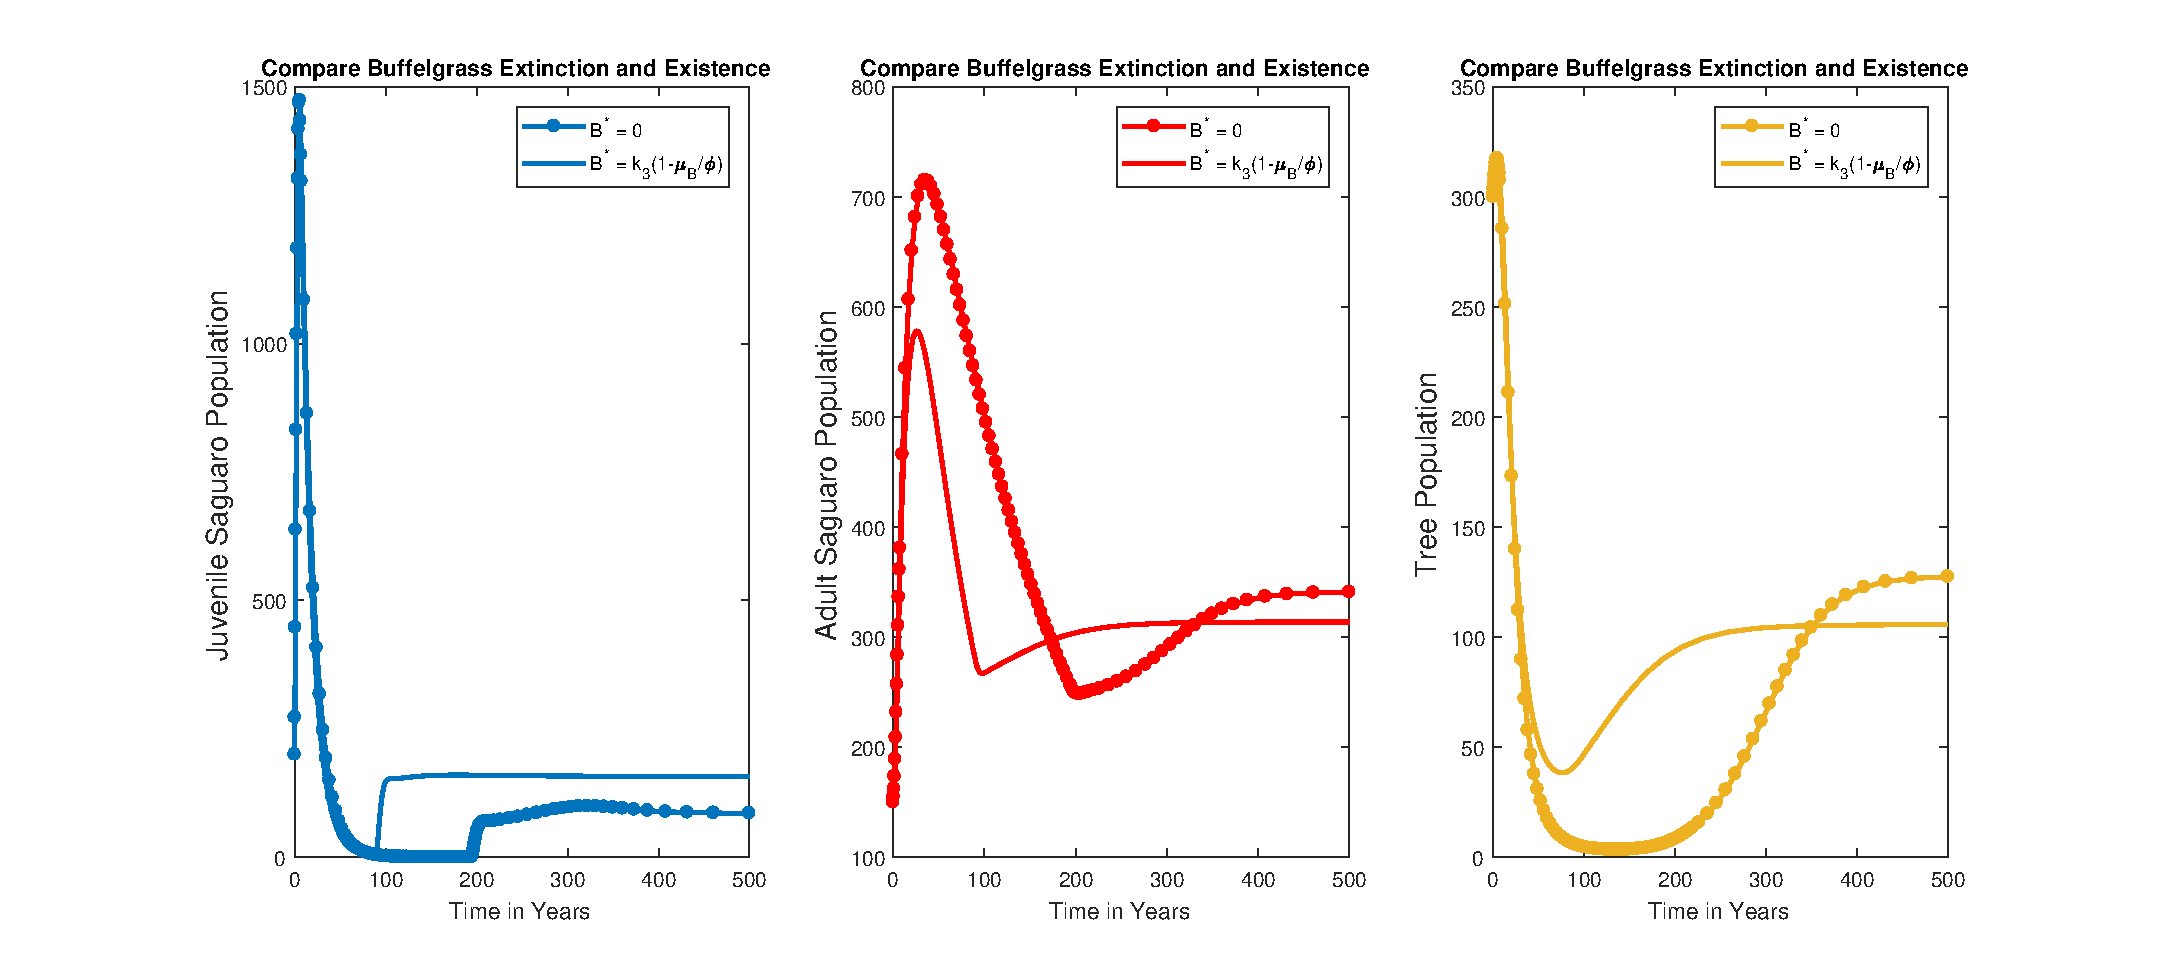
\includegraphics[scale = 0.3]{WandWoutBbyPop.eps}
\end{figure}
\small{Comparing Dynamics at $B^* = 0$ and $B^* = k_3\left(1 - \displaystyle\frac{\mu_B}{\omega}\right)$ equilibria, it can be seen that at $B^* = 0$ equilibrium population values of adult saguaros and  trees are increased.}
\end{frame}

\begin{frame}{Effects of Increased Wildfire Frequency on Equilibrium Populations}
\begin{figure}
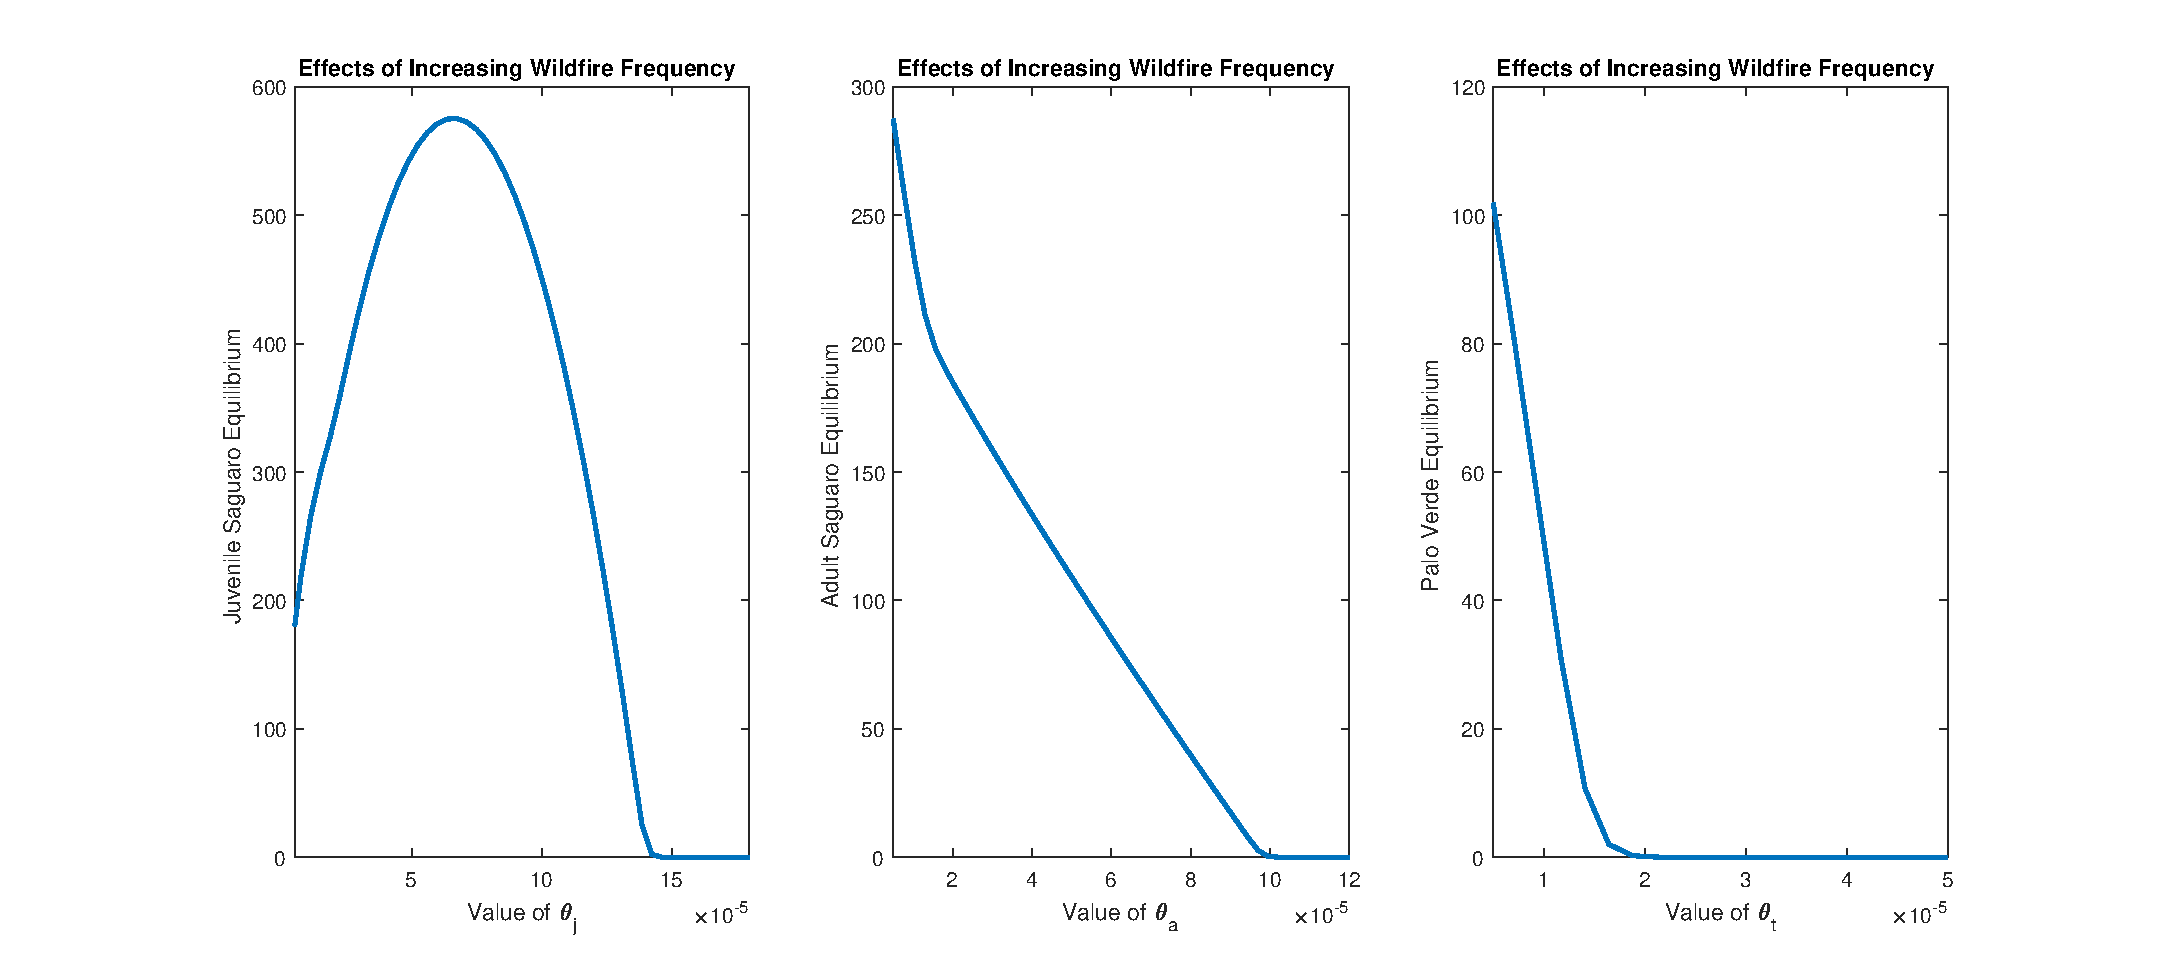
\includegraphics[scale = 0.3]{EqPopVsTheta.eps}
\end{figure}
All equilibrium populations will eventually approach extinction as the frequency of wildfires is increased.
\end{frame}

\begin{frame}{Effects of Increased Wildfire Frequency over Time}
\begin{figure}
{\vspace{-.5cm}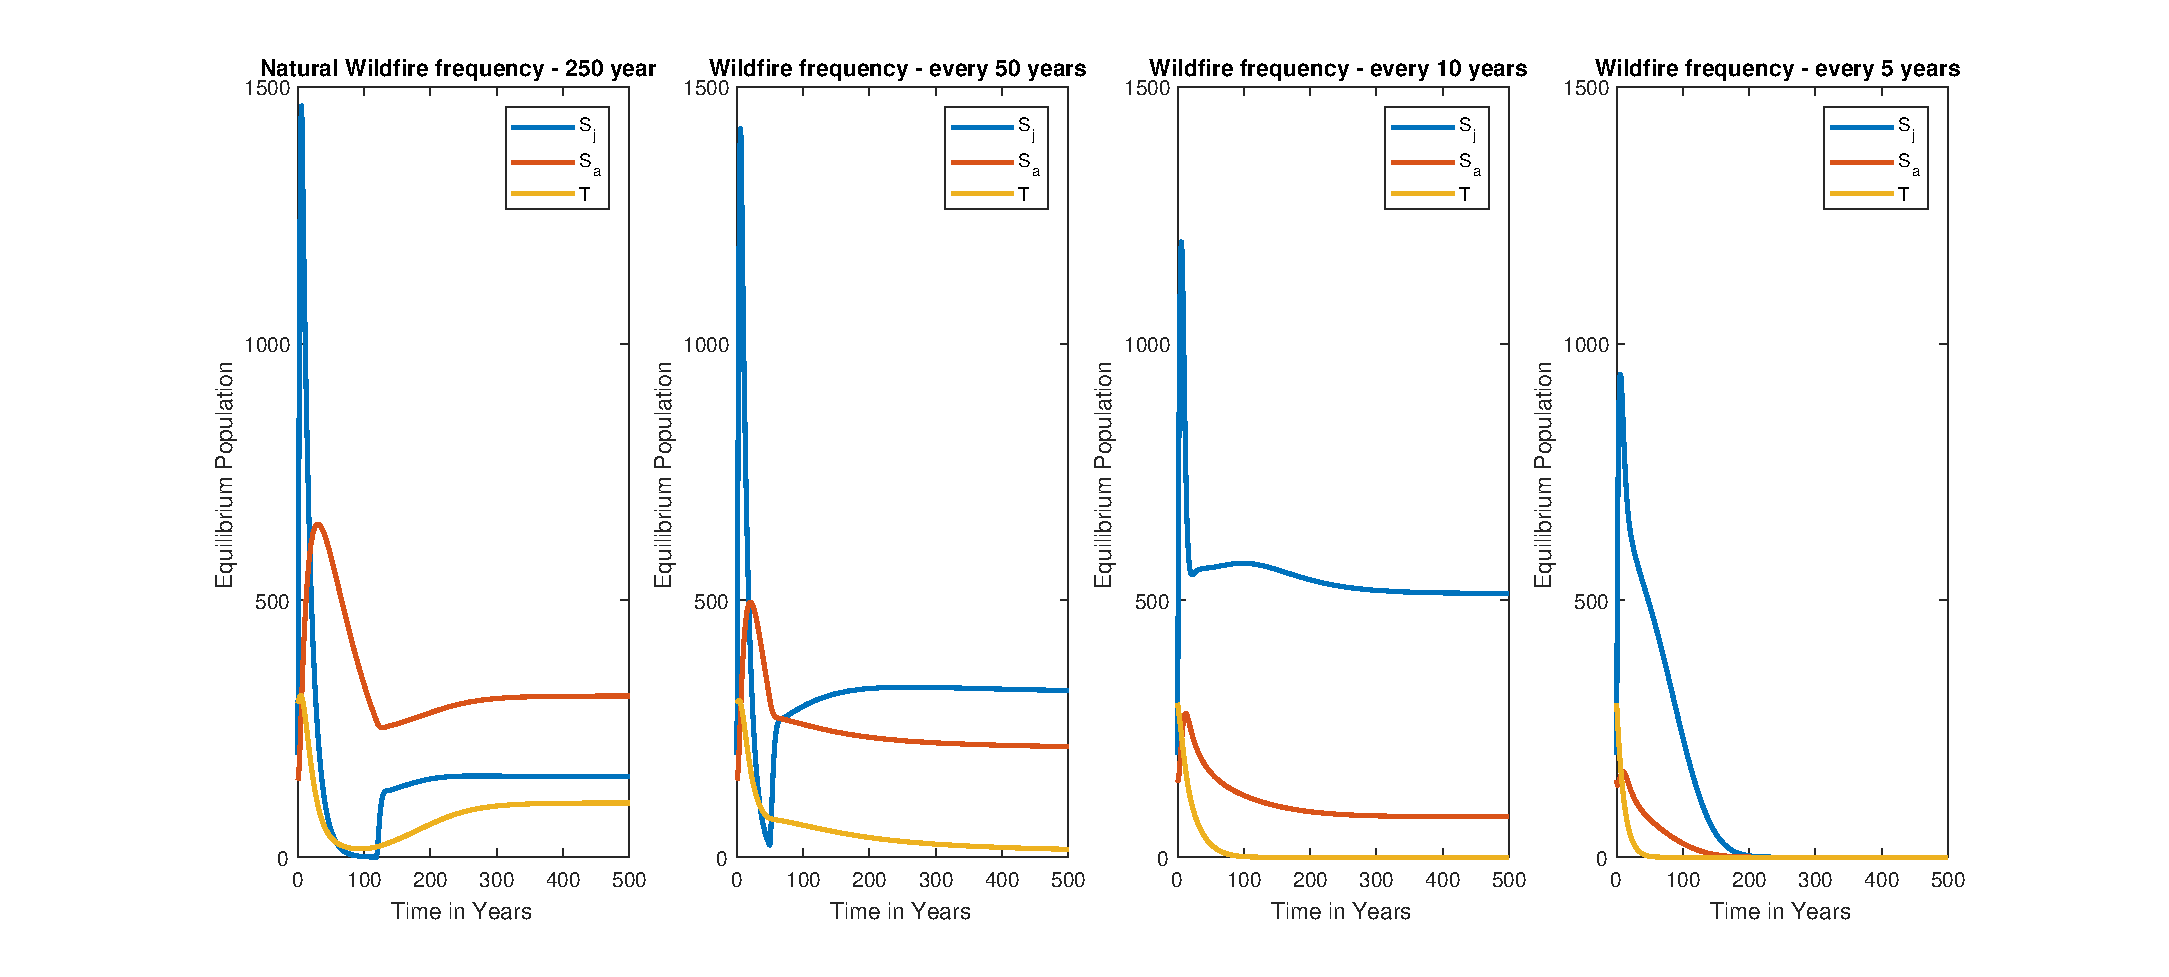
\includegraphics[scale = 0.3]{IncreasingWildfireFrequancy.eps}
}
\vspace{-1cm}
\begin{center}
\begin{minipage}{.2\linewidth}
\tiny{\hspace{.5cm}$\displaystyle\frac{1}{250}$ - Baseline}
\end{minipage}
\begin{minipage}{.25\linewidth}
\tiny{$\displaystyle\frac{1}{50}$ - Real-World Dynamics}
\end{minipage}
\begin{minipage}{.2\linewidth}
\tiny{$\displaystyle\frac{1}{10}$ - Tree Extinction}
\end{minipage}
\begin{minipage}{.2\linewidth}
\tiny{$\displaystyle\frac{1}{5}$ - Saguaro Extinction}
\end{minipage}
\end{center}
\end{figure}
An increase in wildfire frequency can cause the extinction of the saguaros and nurse trees.
\end{frame}

\begin{frame}{Effects of Reducing Buffelgrass by Chemical Spraying}

{\footnotesize \begin{figure}
{\vspace{-.5cm}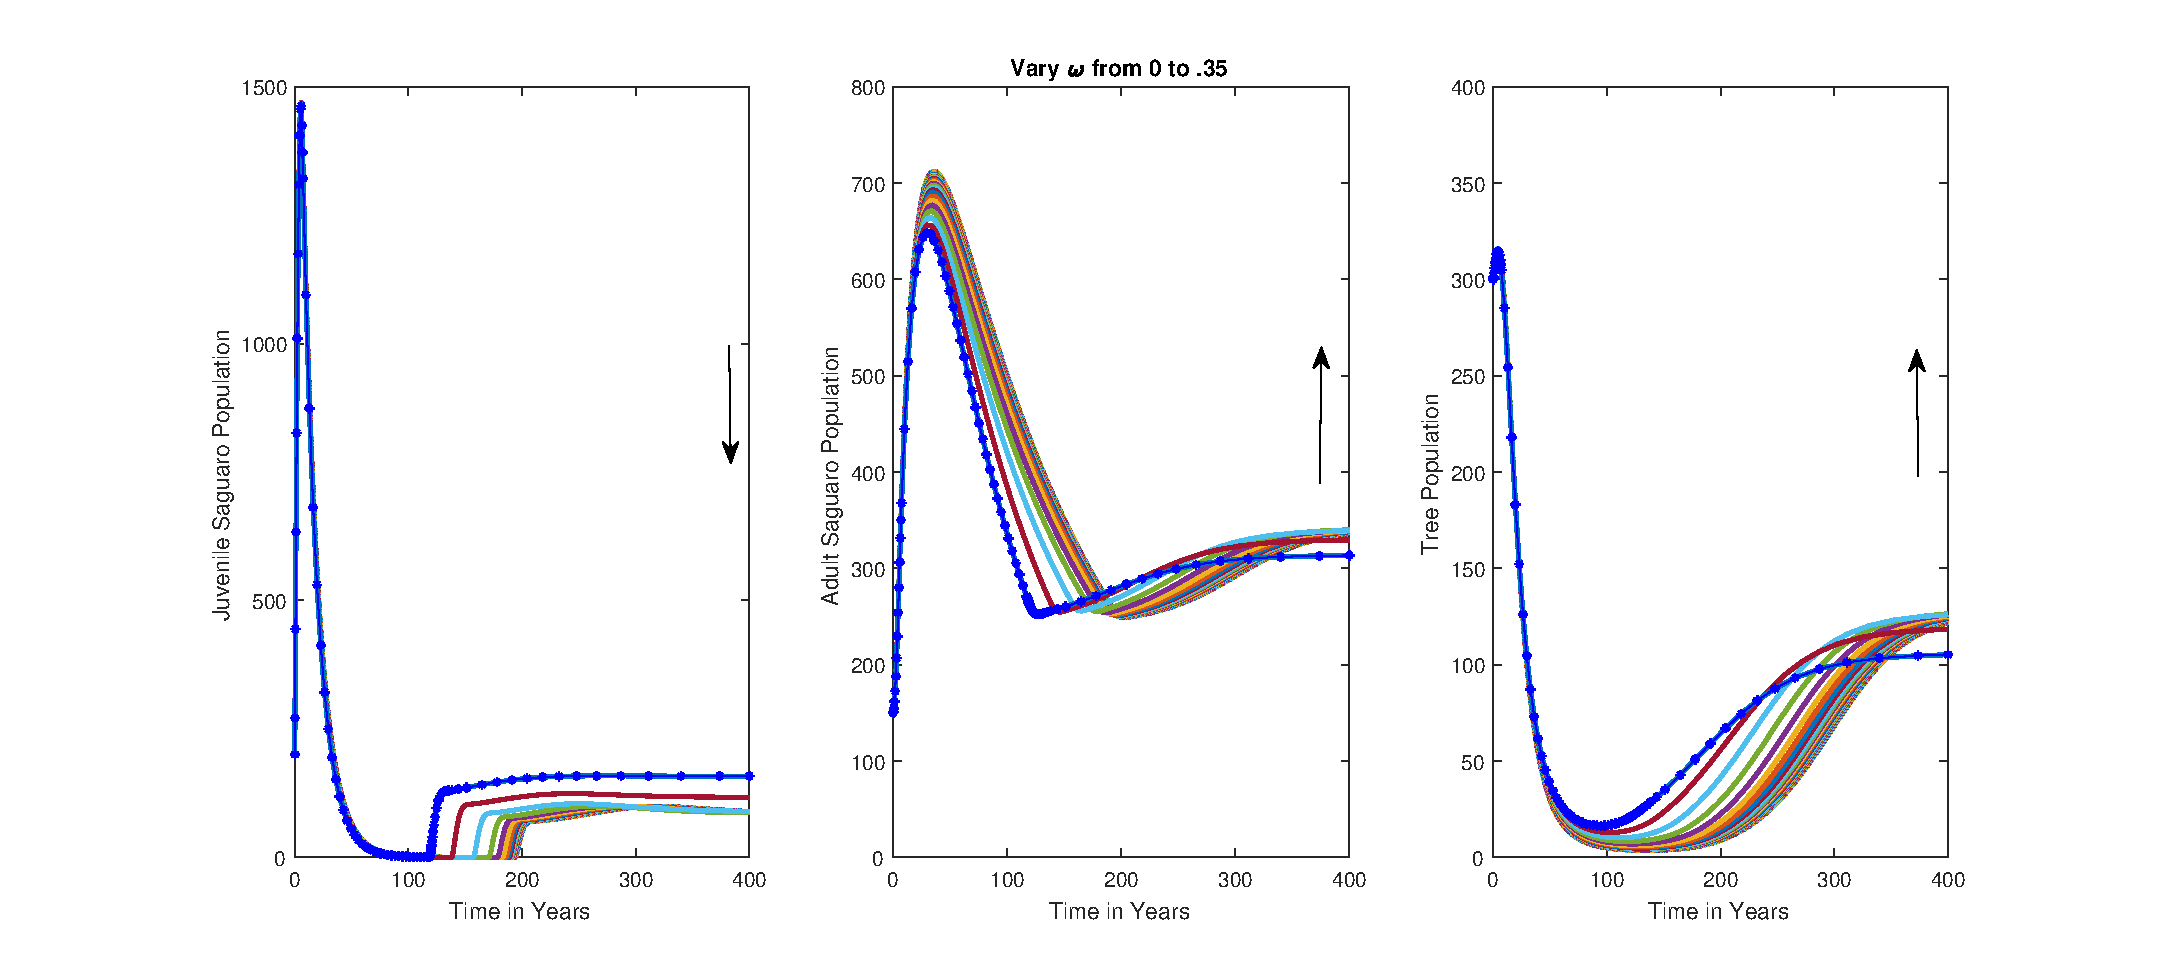
\includegraphics[scale = 0.3]{VaryOmegaWbuffel.eps}}
\end{figure}
The use of herbicide on buffelgrass will increase the adult saguaro and nurse trees population, but it will decrease the juvenile population.} 
\end{frame}


\begin{frame}{Local Sensitivity Analysis Without Buffelgrass}
% Sensitivity analyzed without the inclusion of buffelgrass gives the growth rate of trees, $\phi$, as the most sensitive parameter. This means planting more trees will increase both the nurse tree and saguaro populations the most.\\

\begin{table}
\small{
\begin{center}
\hspace{-.8cm}
\begin{tabular}{|c|c|c|c|c|}\hline
{Sensitivity Analysis}
& $r$ & $b$ & $\phi$\\
\hline
$S_j$ &  0.0013& 0.1006 & 0.6534\\
\hline
$S_a$ & 0.0013 & 0.1006 & 0.6534\\
\hline
$T$ & -0.0084 & -0.6534 & 2.2520\\
\hline
\end{tabular}
\end{center}
}
\end{table}

\end{frame}

\begin{frame}{Local Sensitivity Analysis with Buffelgrass}

%{\footnotesize Sensitivity analysis after the inclusion of buffelgrass shows that the equilibrium populations are most sensitive to the growth rate, $\omega$, and harvesting rate of buffelgrass, $\mu_B$.}\\

\begin{table}
%\centering
\hspace{-.4cm}\small{
\begin{center}
\hspace{-.8cm}
\begin{tabular}{|p{2.8cm}|c|c|c|c|c|}\hline
{Sensitivity Analysis}& $\theta_j$ & $\theta_a$ & $\theta_T$ & $\mu_b$ & $\omega$ \\
\hline
$S_j$ &  \num{-3.92e-04} & 0.4916 & -0.0753 & -8.3189 & 8.3232 \\
\hline
$S_a$ & \num{-3.92e-04} & -0.0111 & -0.0753 & 1.7351
 & -1.7354 \\
\hline
$T$ & 0.0028 & 0.0803 & -0.2980 & 4.2973 & -4.2973\\
\hline
$B$ & N/A & N/A & N/A & -20 & 20\\
\hline
\end{tabular}
 \end{center}
  }
\end{table}
\end{frame}

\begin{frame}{Conclusions}
\small{
\begin{itemize}
\item<1-> Buffelgrass currently coexists with native plants. Fire Frequency thresholds:
\begin{enumerate}
\item<2-> The saguaro population dynamics in the model are similar to real world values if the frequency is at least every 84 years.
\item<3-> Every 24 years leads to nurse tree extinction.
\item<4-> Every 5 years leads to saguaro extinction.
\end{enumerate}
%\item Efforts to reduce buffelgrass should be made to increase available space for the native species and to decrease the rate of wildfire spread.
\item<5-> The most effective way to protect the saguaro population is to decrease the buffelgrass population through the increase of the harvesting rate or decrease of the growth rate.
\begin{enumerate}
\item<6-> Since the sensitivities of the equilibrium populations to these parameters are about the same, which is the more efficient strategy depends on cost.
\end{enumerate}
\end{itemize}}
\end{frame}

\begin{frame}{Future Work}
Future work for this model should be the inclusion of:\\
\begin{itemize}
\item An optimal control analysis for the most efficient way of reducing the buffelgrass population.
\item Adding stochastic wildfires instead of averaging death due to wildfire over time. 
\item Add biological relationships of buffelgrass with native plants
\end{itemize}
\end{frame}

\begin{frame}{Acknowledgements}
\begin{itemize}
\item \small{We would like to thank the Mathematical and Theoretical Biology Institute (MTBI) co-Directors Dr. Carlos Castillo-Chavez, and Dr. Anuj Mubayi for giving us the opportunity to participate in this research program. We would also like to thank associate director Sherry Woodley, coordinator Ciera Duran and management intern Sabrina Avila for their efforts in providing logistics for activities during MTBI.}
\item \small{We also want to give special thanks to our advisors Dr. Karen Ríos-Soto and Dr. Christopher Kribs, and mentors Fan Yu, Juan Melendez-Alvarez, Dr. Leon M Arriola, and Dr. Anuj Mubayi for their contributions throughout this project.}
\item \tiny{The research has been carried out at the MTBI which is a Research Experience for Undergraduate (REU) summer program at the Simon A. Levin Mathematical, Computational and Modeling Sciences Center (SAL MCMSC) at Arizona State University (ASU). This project has been partially supported by grants from the National Science Foundation (DMS1263374), the National Security Agency (H98230-15-1-0021), the Office of the President of ASU, and the Office of the Provost at ASU.}
\end{itemize}
\end{frame}

\begin{frame}
\centering
\huge{Questions?}
\end{frame}

\begin{frame}{Selected Sources}
\bibliographystyle{ieeetr}
\tiny{
\bibliography{bibliography}
\begin{itemize}
\item D. Swann. Personal communication. July 5th 2017.
\end{itemize}}
\end{frame}

\begin{frame}{More Information on Sensitivity Analysis}
A local sensitivity analysis was performed by finding the percent change in the quantity on interest due to a one percent change in the parameter of interest.

$$S_{p}^{q} := \frac{\hat{p}}{\hat{q}} \times \frac{\partial q}{\partial p}\bigg|_{p=\hat{p}} = \frac{\theta_q}{\theta_p}$$

The terms $\hat{p}$ and $\hat{q}$ represent the baseline values of the parameter of interest and quantity of interest, respectively. The $\theta$'s give the changes in the parameter values and resulting changes in quantity values.

\end{frame}
\end{document}

